\documentclass[hyperref={unicode}]{beamer}

%     ITY 2020/2021 Project #5     %
% By Aleksandr Verevkin (xverev00) %

\mode<presentation>
{
  \usetheme{Warsaw}
  \usecolortheme{default}
  \usefonttheme{structurebold}
  \setbeamertemplate{navigation symbols}{}
  \setbeamertemplate{footline}[frame number]
} 

\usepackage[czech]{babel}
\usepackage[utf8]{inputenc}
\usepackage[T1]{fontenc}
\usepackage{lmodern}
\usepackage{listings}
\usepackage{color}
\usepackage[unicode]{hyperref}

\definecolor{dkgreen}{rgb}{0,0.6,0}
\definecolor{gray}{rgb}{0.5,0.5,0.5}
\definecolor{mauve}{rgb}{0.58,0,0.82}

\lstset{frame=tb,
  language=C,
  aboveskip=3mm,
  belowskip=3mm,
  showstringspaces=false,
  columns=flexible,
  basicstyle={\small\ttfamily},
  numbers=none,
  numberstyle=\tiny\color{gray},
  keywordstyle=\color{blue},
  commentstyle=\color{dkgreen},
  stringstyle=\color{mauve},
  breaklines=true,
  breakatwhitespace=true,
  tabsize=3
}

\title{Binární strom}
\author{Aleksandr Verevkin}
\institute{Vysoké učení technické v~Brně\\
Fakulta informačních technologií}


\begin{document}

\begin{frame}
  \titlepage
\end{frame}


\begin{frame}{Obsah}
  \tableofcontents
\end{frame}

\section{Úvod}
\setbeamercovered{transparent}

\begin{frame}{Úvod}

\begin{itemize}
  \item Binární strom je datová struktura,
  používaná k~ukládání a vyhledávání dat v~informatice.
  \pause
  \item Tento typ stromu se používá například pro vyhledávání, reprezentaci zanořených
  seznamových struktur nebo jako vnitřní struktura pro rozhodovací systémy.
\end{itemize}

\end{frame}

\section{Definice struktury}

\subsection{Definice}

\begin{frame}
\frametitle{Definice}
  \begin{columns}
    \begin{column}{.5\textwidth}
     \begin{block}{}
     \begin{center}
        Binární strom se skládá z~uzlů a jednoho kořene (root), 
        ze kterého existuje cesta ke všem uzlům.
    \end{center}
    \end{block}
    \end{column}%
    \begin{column}{.5\textwidth}
    \begin{block}{}
    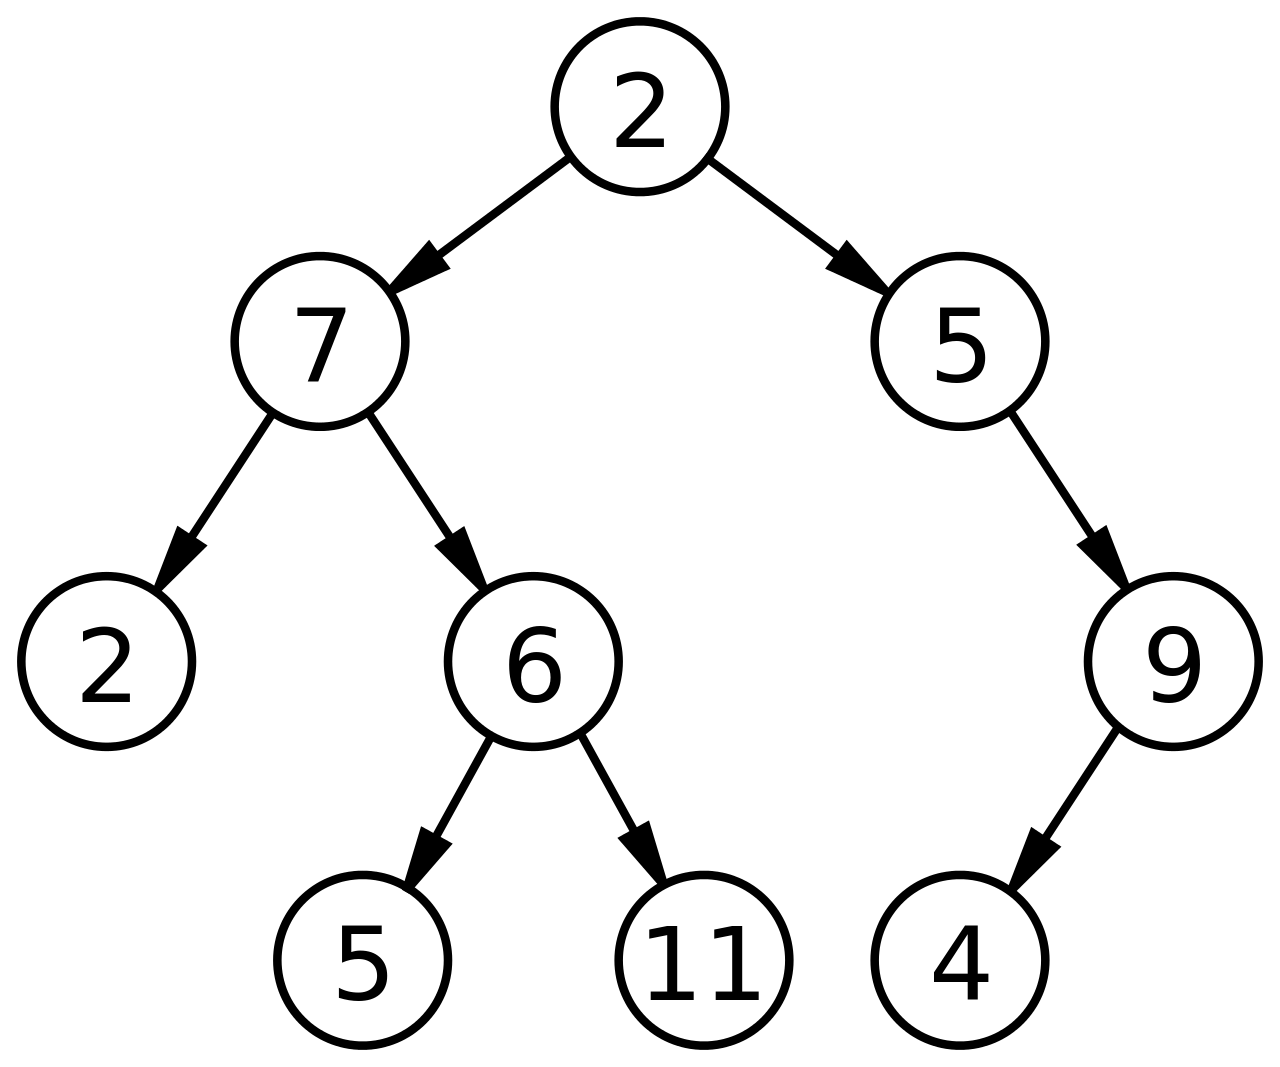
\includegraphics[width=\textwidth]{Binary_tree.png}
    \end{block}
    \end{column}
  \end{columns}
\end{frame} 


\begin{frame}[fragile]{Typy binárních stromů}
\begin{itemize}
    \item \textbf{Binární strom} - obsahuje uzly které mají nejvýš 2 syny.
    \pause
    \item \textbf{Plný binární strom} - každý vnitřní uzel má dva syny.
    \pause
    \item \textbf{Vyvážený binární strom} - hloubka podstromů se od sebe liší maximálně o~jedna.
    \pause
    \item \textbf{Úplný binární strom} - vyvážený binární strom plněný zleva. Jeden poslední vnitřní uzel nemusí být stupně k.
\end{itemize}
\end{frame}

\subsection{Vlastnosti}

\begin{frame}[fragile]{Vlastnosti}
\begin{itemize}
  \item Binární strom má právě jeden kořen (\verb|root|).
  \pause
  \item Každý vrchol binárního stromu může mít maximálně dva orientované syny.
  \pause
  \item Každý vrchol binárního stromu, s~výjimkou kořene, může mít právě jednoho předka.
  \pause
  \item Kořen předka nemá.
\end{itemize}
\end{frame}

\subsection{Implementace}

\begin{frame}[fragile]{Implementace}

\begin{itemize}
    \item V~praktickém programování je obvykle binární strom reprezentován pomocí dynamické struktury,
kde jsou hrany reprezentovány ukazateli.
\end{itemize}

\begin{lstlisting}
typedef struct node {
    int value;            // node value
    struct node *left;    // pointer to the left children
    struct node *right;   // pointer to the right children
} node_t;
\end{lstlisting}

\pause

\begin{itemize}
    \item Implementačně, vrcholy můžou mít též ukazatel na rodiče, kromě dvou ukazatelů na potomky.
\end{itemize}

\end{frame}

\begin{frame}[fragile]{Implementace}

\begin{itemize}
    \item Strom je pak reprezentován kořenem stromu, ze kterého máme
    přístup k~jednotlivým uzlům (potomci \verb|left| a \verb|right|).
\end{itemize}

\vskip 1cm

\begin{lstlisting}
node_t *tree;           // tree
node_t *tree.left;      // left children
node_t *tree.right;     // right children
\end{lstlisting}

\end{frame}

\begin{frame}[fragile]{Implementace}
\begin{itemize}
    \item Při vložení prvku dynamicky alokujeme uzel pomocnou funkcí
    (v našem případě \verb|newNode()|).
\end{itemize}

\vskip 0.5cm

\begin{lstlisting}
node_t* newNode(int value) {
    node_t *node= (node_t*)malloc(sizeof(node_t));
    node->value = value;            // prirazeni hodnoty
    node->left = node->right = NULL;
    return node; 
}
\end{lstlisting}

\end{frame}

\section{Literatura}

\subsection{Seznam použité literatury}

\begin{frame}{Seznam použité literatury}

\begin{thebibliography}{9}
\bibitem{voho} HORDĚJČUK Vojtěch: \emph{Binární strom (binary tree).}\\
Dostupně z: \href{http://voho.eu/wiki/datova-struktura-strom/}
{http://voho.eu/wiki/datova-struktura-strom/}
\bibitem{faigl} FAIGL Jan: \emph{Stromy.}\\
Dostupně z: \href{https://cw.fel.cvut.cz/old/_media/courses/b0b36prp/lectures/b0b36prp-lec10-slides.pdf}
{https://cw.fel.cvut.cz/old/\_media/courses/\\
b0b36prp/lectures/b0b36prp-lec10-slides.pdf}
\end{thebibliography}
\end{frame}

\end{document}
